\documentclass[14pt]{extarticle}

\usepackage[utf8]{inputenc}
\usepackage[english,ukrainian]{babel}
\usepackage{bookmark}
\usepackage{libertine}

\usepackage{amsmath,amssymb}
\usepackage{parskip}
\usepackage{graphicx}
\usepackage[table]{xcolor}
\usepackage{tcolorbox}
\tcbuselibrary{skins}
\usepackage[framemethod=tikz]{mdframed}
\usepackage{chngcntr}
\usepackage{enumitem}
\usepackage{hyperref}
\usepackage{float}
\usepackage{subfig}
\usepackage{chngcntr}
\usepackage{esint}
\usepackage{pdfpages} % Add this to your preamble

\usepackage[cache=false]{minted}
\usemintedstyle{tango}

\usepackage{libertinus}
\renewcommand\ttdefault{cmtt}

\usepackage[top=2.5cm, left=3cm, right=3cm, bottom=4.0cm]{geometry}
\usepackage{algorithm}
\usepackage{algpseudocode}
\usepackage{listings}
\usepackage{xcolor}

\definecolor{codegreen}{rgb}{0,0.6,0}
\definecolor{codegray}{rgb}{0.5,0.5,0.5}
\definecolor{codepurple}{rgb}{0.58,0,0.82}
\definecolor{backcolour}{rgb}{0.95,0.95,0.92}

\lstdefinestyle{mystyle}{
    backgroundcolor=\color{backcolour},   
    commentstyle=\color{codegreen},
    keywordstyle=\color{magenta},
    numberstyle=\tiny\color{codegray},
    stringstyle=\color{codepurple},
    basicstyle=\ttfamily\footnotesize,
    breakatwhitespace=false,         
    breaklines=true,                 
    captionpos=b,                    
    keepspaces=true,                 
    numbers=left,                    
    numbersep=5pt,                  
    showspaces=false,                
    showstringspaces=false,
    showtabs=false,                  
    tabsize=2
}
\lstset{style=mystyle}

\usepackage{ragged2e}
\begin{document}

\begin{titlepage}
	\centering
	%
\includegraphics[width=0.15\textwidth]{images/lab_1/logo.png}\par\vspace{0.3cm}
	{\textbf{Міністерство освіти і науки України}\par
 Харківський національний університет імені В.Н. Каразіна\par}
    \vspace{1cm}
	{\Large \textsc{Розрахунково-графічне завдання \#3}\par
    \textbf{Чисельне розв'язання рівнянь із частинними похідними}\par}
	\vfill
 \begin{FlushRight}
	\textbf{Виконав:}\par Захаров Дмитро Олегович \par Група МП-41
\end{FlushRight}
	\vfill

% Bottom of the page
	{\large Харків -- 2025\par}
\end{titlepage}

\tableofcontents
\pagebreak

\section{Постановка задачі}

Для розв'язання завдання використати або метод прямих (диференціально-сітковий)
метод або метод сіток. Перевірити точність можна з використанням подвійного
перерахунку. Диференціальне рівняння:
\begin{equation*}
    \Delta u(x,y) - \sin x \cdot u(x,y) = 20[x+y]^2, \quad 0 < x < a, \quad 0 < y < b 
\end{equation*}

для заданих граничних умов
\begin{equation*}
    (u_{\nu}+u)\Big|_{x=0} = 0, u\Big|_{x=a} = 0, \quad (u_{\nu}+u)\Big|_{y=0} = 0, u\Big|_{y=b} = 0
\end{equation*}

із точністю $\varepsilon = 10^{-3}$. Тут $a=2$, $b=1$, $u_{\nu}$ --- похідна 
по зовнішній нормалі до границі області. Надрукувати розв'язок у вигляді 
таблиці $10 \times 10$. 

\pagebreak
\section{Опис методів}

\subsection{Метод прямих}

Головна ідея методу прямих полягає в зведенні рівняння в частинних похідних 
до системи звичайних диференціальних рівнянь. Нехай маємо диференціальне 
рівняння другого порядку у двох змінних:
\begin{equation*}
    \Delta u + f(x,y)u = g(x,y), \quad (x,y) \in \Omega = (0,a) \times (0,b)
\end{equation*}

Зафіксуємо певний $n \in \mathbb{N}$
(в нашому конкретному випадку $n=10$) та розглянемо крок $h := \frac{a}{n}$
вздовж осі $x$. Тоді розглянемо функції $u_i(y) := u(x_i,y)$ для 
$i \in [n]$ та $x_i = ih$, $i=0,\dots,n$. Скористаємось наближеннями 
для похідних за $x$ (вважаємо, що крок $h$ достатньо малий):
\begin{equation*}
    \nabla u(x_i,y) = \frac{\partial^2 u(x_i,y)}{\partial x^2} + \frac{\partial^2 u(x_i,y)}{\partial y^2} \approx \frac{u_{i-1}(y) - 2u_i(y) + u_{i+1}(y)}{h^2} + \frac{d^2u_i}{dy^2}
\end{equation*}

Тоді отримаємо систему звичайних диференціальних рівнянь:
\begin{equation*}
    \frac{u_{i-1}(y) - 2u_i(y) + u_{i+1}(y)}{h^2} + \frac{d^2u_i}{dy^2} + f(x_i,y)u_i(y) = g(x_i,y), \quad i \in [n]
\end{equation*}

з відповідними граничними умовами. Такий спосіб доволі складний, оскільки вимагає 
розв'язок $n$ звичайних диференціальних рівнянь другого порядку (що \textit{Wolfram Mathematica}
у її безкоштовній версії не дозволяє через обмеження ресурсів). Тому 
замість цього скористаємося методом сіток.

\subsection{Метод сіток}

Знову нехай маємо рівняння другого порядку у двох змінних:
\begin{equation*}
    \begin{cases}
        \Delta u + f(x,y)u = g(x,y), \quad (x,y) \in \Omega = (0,a) \times (0,b) \\
        (u_{\nu}+u)\Big|_{x=0} = u\Big|_{x=a} = (u_{\nu}+u)\Big|_{y=0} = u\Big|_{y=b} = 0
    \end{cases}
\end{equation*}

\textcolor{blue}{\textbf{Рівняння в дискретній формі.}} Тепер дискретизацію
області $\Omega$ виконаємо у двох напрямках. Нехай $n$ це щільність сітки у обох
напрямках, тоді отримаємо сітку з $(n+1)^2$ вузлів. Значення функції $u(x_i,y_i)$ у
вузлі $(x_i,y_i)=(\frac{ia}{n},\frac{ib}{n})$ позначимо через $u_{i,j}$. Тоді
апроксимація оператора Лапласа у точці $(x_i,y_j)$ має наступний вигляд:
\begin{equation*}
    \Delta u(x_i,y_j) \approx \frac{u_{i-1,j} - 2u_{i,j} + u_{i+1,j}}{h_x^2} + \frac{u_{i,j-1} - 2u_{i,j} + u_{i,j-1}}{h_y^2},
\end{equation*}

де $h_x = \frac{a}{n}$, $h_y = \frac{b}{n}$. Тоді, підставивши це у рівняння, отримаємо для кожного вузла $(i,j)$ наступне рівняння:
\begin{equation*}
    \textcolor{blue}{\frac{u_{i-1,j} - 2u_{i,j} + u_{i+1,j}}{h_x^2} + \frac{u_{i,j-1} - 2u_{i,j} + u_{i,j-1}}{h_y^2} - f(ih_x,jh_y)u_{i,j} = g(ih_x,jh_y)}
\end{equation*}

\textcolor{green!50!black}{\textbf{Граничні умови.}} Залишилось виписати
граничні умови на мові дискретизованих значень. Умова $u(a,y) \equiv u(x,b)
\equiv 0$ інтерпретується дуже просто:
\begin{equation*}
    \textcolor{green!50!black}{u_{n,j} = 0, \quad u_{i,n} = 0, \quad i,j \in [n]}
\end{equation*}

Розглянемо умову $(u_{\nu}+u)(0,y) = 0$. Оскільки $\nu=(-1,0)$ за $x=0$,
то маємо $-\frac{\partial u}{\partial x}(0,y) + u(0,y) = 0$. Апроксимуємо 
похідну за $x$:
\begin{equation*}
    -\frac{\partial u}{\partial x}(0,y_j) + u(0,y_j) \approx -\frac{u_{1,j} - u_{0,j}}{h_x} + u_{0,j} = 0 \implies \textcolor{green!50!black}{(1+h_x)u_{0,j} = u_{1,j}, j \in [n]}
\end{equation*}

Нарешті, умова $(u_{\nu}+u)(x,0) = 0$ інтерпретується аналогічно:
\begin{equation*}
    \textcolor{green!50!black}{(1+h_y)u_{i,0} = u_{i,1}, \quad i \in [n]}
\end{equation*}

\textcolor{purple}{\textbf{Система лінійних рівнянь.}} Отже, ми отримали систему
\begin{equation*}
    \begin{cases}
        \frac{u_{i-1,j} - 2u_{i,j} + u_{i+1,j}}{h_x^2} + \frac{u_{i,j-1} - 2u_{i,j} + u_{i,j-1}}{h_y^2} + f(ih_x,jh_y)u_{i,j} = g(ih_x,jh_y), \\
        (1+h_x)u_{0,j} = u_{1,j}, \quad (1+h_y)u_{i,0} = u_{i,1}, \quad u_{n,j} = 0, \quad u_{i,n} = 0
    \end{cases}
\end{equation*}

Це є системою лінійних рівнянь відносно $(n+1)^2$ невідомих. В нашому випадку,
ми просто акуратно випишемо матрицю системи та вектор правих частин, а потім
скористаємося стандартними методами розв'язання системи лінійних рівнянь (скажімо,
ітеративними). Звичайно, оскільки матриця є розрідженою, то існують значно 
більш ефективні алгоритми розв'язання таких систем, але ми не будемо
надто ускладнювати задачу (особливо для $n=10$).

\section{Імплементація}

\subsection{Код функції розв'язку}

Знизу ми наводимо код функції, що реалізує описаний вище алгоритм.

\begin{minted}{python}
from typing import Callable

# Some math-related imports
import numpy as np
from scipy.sparse import lil_matrix
from scipy.sparse.linalg import spsolve


def solve_pde(
    n: int, 
    a: float, 
    b: float, 
    f_func: Callable[[np.ndarray], np.ndarray], 
    g_func: Callable[[np.ndarray], np.ndarray]
) -> np.ndarray:
    """
    Solves the PDE:
        nabla u + f(x,y)*u = g(x,y)
    with boundary conditions:
        (du/dn + u)|_{x=0, y=0} = 0
        u|_{x=a, y=b} = 0
        
    Parameters:
        n: number of interior points per axis (grid is (n+1)x(n+1))
        a, b: domain size in x and y
        f_func: function f(x, y)
        g_func: function g(x, y)
        
    Returns:
        u: (n+1)x(n+1) array with solution values on the grid
    """
    
    h_x = a / n # Grid size in x direction
    h_y = b / n # Grid size in y direction
    N = (n+1) ** 2  # Total number of points (including boundaries)
    
    A = lil_matrix((N, N)) # Sparse matrix for the system
    b_vec = np.zeros(N) # Right-hand side vector

    def idx(i: int, j: int) -> int:
        """
        Returns the flattened index for the 2D grid.
        """
        return i * (n + 1) + j

    for i in range(n+1):
        for j in range(n+1):
            x, y = i * h_x, j * h_y # Calculate the coordinates
            k = idx(i, j) # Flattened index for the matrix
            f_val = f_func(x, y)
            g_val = g_func(x, y)

            # Boundary for x=a or y=b
            if i == n or j == n:
                A[k, k] = 1.0
                b_vec[k] = 0.0

            # Boundary for x=0 or y=0
            elif i == 0 and j < n:
                kp = idx(i + 1, j)
                A[k, k] = 1 + h_x
                A[k, kp] = -1
                b_vec[k] = 0.0
            elif j == 0 and i < n:
                kp = idx(i, j + 1)
                A[k, k] = 1 + h_y
                A[k, kp] = -1
                b_vec[k] = 0.0

            # Now, the main part of the grid
            else:
                xm = idx(i - 1, j)
                xp = idx(i + 1, j)
                ym = idx(i, j - 1)
                yp = idx(i, j + 1)

                A[k, k] = -2 / h_x**2 - 2 / h_y**2 + f_val
                A[k, xm] = 1 / h_x**2
                A[k, xp] = 1 / h_x**2
                A[k, ym] = 1 / h_y**2
                A[k, yp] = 1 / h_y**2

                b_vec[k] = g_val

    u_flat = spsolve(A.tocsr(), b_vec)
    return u_flat.reshape((n + 1, n + 1))
\end{minted}

Нарешті, використаємо наступний код, щоб відобразити результат, а також перевірити різницю згідно подвійного перерахунку.

\begin{minted}{python}
from solver import solve_pde

import numpy as np

# For visualization
import matplotlib.pyplot as plt


if __name__ == "__main__":
    # First, solve the equation
    a, b = 2.0, 1.0
    n = 30
    f_func = lambda x, y: np.sin(x)
    g_func = lambda x, y: 20 * np.round(x+y)**2
    
    u_solution = solve_pde(n, a, b, f_func, g_func)
    u_solution_2n = solve_pde(2*n, a, b, f_func, g_func)
    
    # Validate that the difference between the two solutions is small
    diff = np.max(np.abs(u_solution - u_solution_2n[::2, ::2]))
    print(f"Max difference between n={n} and n={2*n} solutions: {diff:.2e}")

    x = np.linspace(0, a, n + 1)
    y = np.linspace(0, b, n + 1)
    X, Y = np.meshgrid(x, y, indexing="ij")
    
    # Contour plot with colorbar (already done)
    plt.figure(figsize=(6, 5))
    plt.contourf(X, Y, u_solution, levels=50, cmap="viridis")
    plt.colorbar(label="u(x,y)")
    plt.title("Solution to the PDE")
    plt.xlabel("x")
    plt.ylabel("y")
    plt.tight_layout()
    plt.savefig("contour_plot.pdf", dpi=300)
    plt.show()
    
    # 3D surface plot
    fig = plt.figure(figsize=(8, 6))
    ax = fig.add_subplot(111, projection='3d')
    surf = ax.plot_surface(X, Y, u_solution, cmap='viridis', edgecolor='none')
    fig.colorbar(surf, ax=ax, shrink=0.5, aspect=10, label="u(x,y)")
    ax.set_title("Surface Plot of the Solution")
    ax.set_xlabel("x")
    ax.set_ylabel("y")
    ax.set_zlabel("u(x,y)")
    plt.tight_layout()
    plt.savefig("surface_plot.pdf", dpi=300)
    plt.show()
\end{minted}

Отримаємо, що максимальна різниця менша за $\varepsilon$, тому побудований розв'язок доволі точний (нормальну точність досягнуто за $n=30$). 

Самі розв'язки проілюстровано на Рисунку \ref{fig:with_friction}.

\begin{figure}[H]
    \begin{tabular}{cc}
      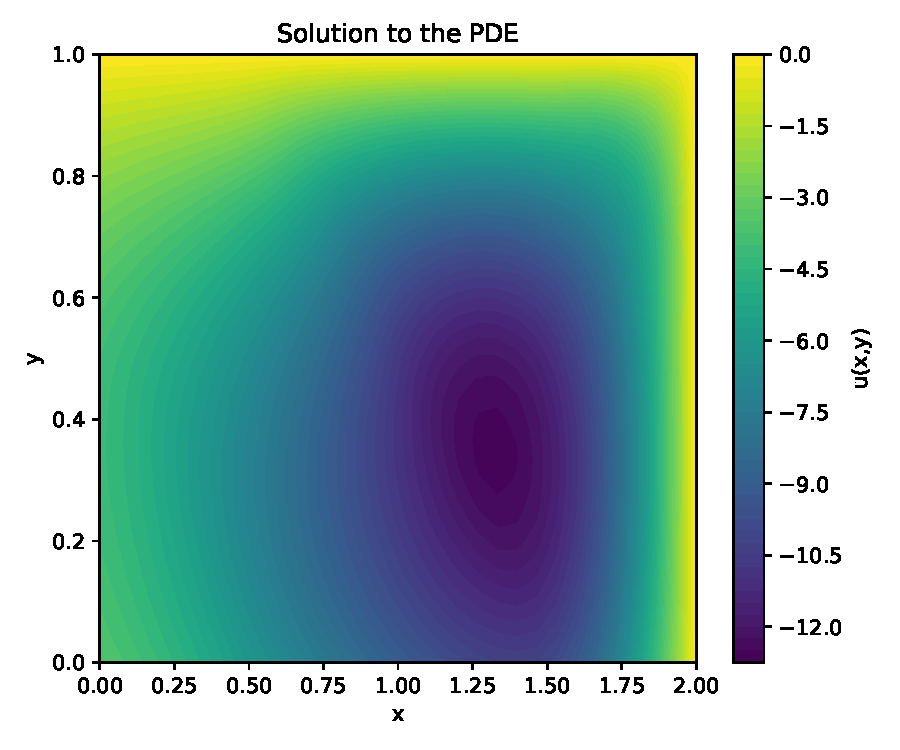
\includegraphics[width=0.5\textwidth]{appendices/homework_3/contour_plot.pdf} &   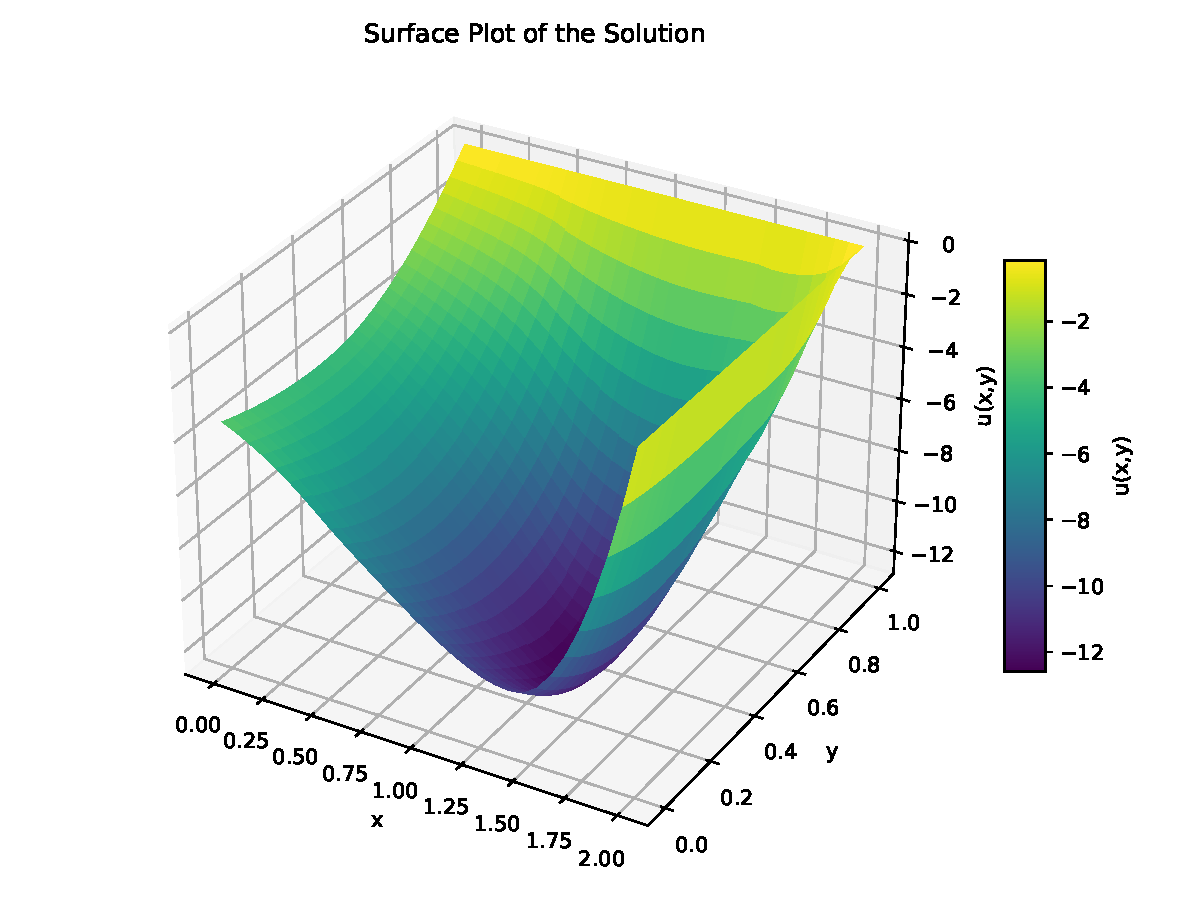
\includegraphics[width=0.5\textwidth]{appendices/homework_3/surface_plot.pdf} \\
      Contour Plot & Surface Plot
    \end{tabular}
    \caption{Розв'язки заданого рівняння.}
    \label{fig:with_friction}
\end{figure}

\end{document}

